\subsection{Systematiske test (black box test) (Roar)}

\iffalse
\begin{mdframed}[backgroundcolor=black!5]
Dette afsnit skal indeholde planer for systematiske
tests til udvalgte use case scenarier nævnt i afsnit use cases ved brug af systematiske test metoden for black box test (jf. slides uge 5). \

I det mindste dog alle scenarier til 2  use cases for tomandsgrupper, 3 for tremandsgrupper og 4 for firmandsgrupper. Benyt samme skabelon til systematiske tests som er brugt i forbindelse med forelæsninger (dvs. to tabeller; den ene med input egenskaber og den anden med konkrete værdier).\\

Hvis de valgte use cases og deres scenarier har ændret sig fra versionen i rapport 1, så skal de aktuelle use cases og deres scenarier vises igen i den ændret version i rapport 2. De planlagte systematiske test skal implementeres og udføres ved brug af JUnit og skal afleveres som en del af Eclipse projektet. \\

Desuden skal testene demonstreres i programdemoen på Mandag den 8 maj. \\

Ydeligere skal rapport 2 have et diagram som viser code coverage af de enkelte Java filer efter alle testene er kørt, sammen med en forklaring af code coverages resultater. \end{mdframed}
\fi

Black box testing er et kraftigt værktøj mht. at teste et program. Teknikken går ud på at teste et program udefra, og kræver ikke stor indsigt i hvordan programmet virker bag facaden. Under black box testing bestemmer man præmisserne og evaluerer om resultatet/outputtet er korrekt. I dette tilfælde er det ikke return-statements der bliver evalueret, da de fleste metoder i programmet ikke virker ved at returnere en værdi. I stedet er det den interne datastruktur der bliver verificeret. \\

De black box tests der vil blive kigget på her, tager udgangspunkt i 4 af de mest essentielle use cases programmet er bygget på. Da det er den interne datastruktur der tjekkes, vil testene bruge informationer fra den sampledata der sættes op i \texttt{App}'s konstruktør.

De use cases vi vil kigge på, er:
\begin{enumerate}
    \item Melde timer på aktivitet.
    \item Anmode om medlemmer til aktivitet.
    \item Valg af projektleder.
    \item Ændring af status.
\end{enumerate} 
\vspace{3mm}

Nogle af de brugte use cases er ændret siden rapport 1, hvor de opdaterede versioner ses inden testen præsenteres. Testene vil blive præsenteret ved brug af 2 tabeller (som i forelæsningerne fra uge 5). Først vil en tabel blive vist med datasæt og egenskaberne af sættene. Disse sæt repræsenterer til sammen alle mulige/legale input. Derefter vil en tabel blive vist med de samme datasæt, denne gang med konkrete værdier fra datasættene og det forventede resultat af testen. \\

Til hver test findes der JUnit test filer der tjekker at testen godkendes i programmet. Værdierne i testene i rapporten stemmer så vidt muligt overens med værdierne i JUnit testene. \\

\subsubsection{Melde timer på aktivitet}

Denne use case er ikke ændret siden rapport 1.

\begin{table}[H]
    \centering
    \begin{tabular}{|l|l|}
    \hline
    \textbf{Input} & \textbf{Egenskab}                                                                   \\ \hline
 A     & Bruger i aktiviteten melder  ml. 0 og 24 timer på ny dato                   \\ \hline
    B     & Bruger ikke i aktiviteten melder ml. 0 og 24 timer på ny dato               \\ \hline
    C     & Bruger i aktiviteten melder over 24 timer på ny dato                        \\ \hline
    D     & Bruger i aktiviteten melder under 0 timer på ny dato                        \\ \hline
    E     & Bruger i aktiviteten melder ml. 0 og 24 timer på dato allerede registreret  \\ \hline
    \end{tabular}
\end{table}

Metoden til at registrere timer ligger i \texttt{Employee} klassen. Metoden tager 3 parametre: dato, aktivitet og antal timer. Værdierne i kolonnen for "Konkrete værdier" i nedenstående tabel følger den nævnte rækkefølge.

\begin{table}[H]
    \centering
    \begin{tabular}{|l|l|l|}
    \hline
    \textbf{Input} &     \textbf{Konkrete værdier}              & \textbf{Resultat}                       \\ \hline
    A     & Victor, 125/2017, Optional Activity, 6  & 6 timer er registreret    \\ \hline
    B     & Victor, 125/2017, Master Activity, 2    & Ingen registrering        \\ \hline
    C     & Victor, 125/2017, Optional Activity, 25 & Ingen registrering        \\ \hline
    D     & Victor, 125/2017, Optional Activity, -1 & Ingen registrering        \\ \hline
    E     & Victor, 020/2017, Optional Activity, 5  & 5 timer registreret       \\ \hline
    \end{tabular}
    
\end{table}

JUnit tests kan ses i filerne: \\
\texttt{TestEmployeeRegisterHoursOnActivity} \\ 
\texttt{TestEmployeeEditHours}. \\

\subsubsection{Anmode om medlemmer til aktivitet}

Denne use case er ændret siden rapport 1:

\textbf{Navn:} Anmode om medlemmer til aktiviteter.

\textbf{Aktør:} Medarbejder.

\textbf{Forudsætning:} Brugeren er tilmeldt aktiviteten.
    
\textbf{Hovedscenarie: }
    
\begin{itemize}
    \item Brugeren vælger den gældende aktivitet.
    \item Brugeren anmoder om hvem der skal tilmeldes aktiviteten.
    \item Systemet tilføjer den gældende bruger til aktiviteten.
\end{itemize}

\textbf{Alternativt scenarie:}
\begin{itemize}
    \item Brugeren findes allerede i aktiviteten
    \item Brugeren forbliver i aktiviteten
\end{itemize}

\textbf{Alternativt scenarie:}
\begin{itemize}
    \item Brugeren findes ikke i systemet
    \item Brugeren bliver ikke tilføjet til aktiviteten
\end{itemize}

\textbf{Alternativt scenarie:}
\begin{itemize}
    \item Aktiviteten findes ikke i systemet
    \item Brugeren bliver ikke tilføjet til aktiviteten
\end{itemize}

\vspace{1cm}

Der er tilføjet flere alternative scenarier, og det kræves ikke at projektlederen skal bekræfte anmodningen for at brugeren tilføjes til aktiviteten.

\begin{table}[H]
    \centering
    \begin{tabular}{|l|l|}
    \hline
    \textbf{Input} & \textbf{Egenskab}                                                        \\ \hline
    A     & Bruger i systemet anmodet til aktivitet brugeren ikke er i      \\ \hline
    B     & Bruger i systemet anmodet til aktivitet brugeren er i           \\ \hline
    C     & Bruger ikke i systemet anmodet til aktivitet brugeren ikke er i \\ \hline
    D     & Bruger i systemet anmodet til aktivitet ikke i systemet         \\ \hline
    \end{tabular}
\end{table}

Metoden til at anmode om medlemmer til aktiviteter kræver to parametre: bruger og aktivitet. Værdierne i kolonnen for "Konkrete værdier" i nedenstående tabel følger den nævnte rækkefølge.

\begin{table}[H]
    \centering
    \begin{tabular}{|l|l|l|}
    \hline
    \textbf{Input} &     \textbf{Konkrete værdier}              & \textbf{Resultat}                        \\ \hline
    A     & Victor, ny aktivitet  & Victor er tilføjet til den nye aktivitet    \\ \hline
    B     & Victor, Optional Activity    & Victor er ikke tilføjet igen         \\ \hline
    C     & Ukendt bruger, Optional Activity & Brugeren er ikke tilføjet        \\ \hline
    D     & Victor, ukendt aktivitet & Victor er ikke tilføjet                  \\ \hline

    \end{tabular}
    
\end{table}

JUnit tests kan ses i filen: \\
\texttt{TestEmployeeAssist}.


\subsubsection{Valg af projektleder}

Denne use case er ændret siden rapport 1:

\textbf{Navn:} Valg af projektleder

\textbf{Aktør:} Medarbejder.


\textbf{Hovedscenarie: }
    
\begin{itemize}
    \item Projektet har ingen leder.
    \item Brugeren vælger hvilken medarbejder der er projektleder.
    \item Den valgte medarbejder er registreret som projektleder.
\end{itemize}

\textbf{Alternativt scenarie:}
\begin{itemize}
    \item Brugeren er projektleder.
    \item Brugeren vælger hvilken medarbejder der er projektleder.
    \item Medarbejderen bliver gjort til projektleder.
\end{itemize}

\textbf{Alternativt scenarie:}
\begin{itemize}
    \item Projektet har en leder.
    \item Brugeren er ikke projektleder.
    \item Brugeren vælger hvilken medarbejder der er projektleder.
    \item Medarbejderen bliver ikke gjort til projektleder.
\end{itemize}

\vspace{1 cm}

Alle kan tilføje en projektleder til et projekt hvis der ingen projektleder er. Hvis der findes en projektleder er det kun projektlederen der kan vælge den nye leder.

\begin{table}[H]
    \centering
    \begin{tabular}{|l|l|}
    \hline
    \textbf{Input} & \textbf{Egenskab}                                                            \\ \hline
    A     & Ingen projektleder. En bruger vælger en ny leder                    \\ \hline
    B     & Projektleder findes. En bruger vælger en ny leder                   \\ \hline
    C     & Projektleder findes. Lederen vælger en ny leder                     \\ \hline
    D     & Ingen projektleder. En bruger vælger en ny leder ikke i systemet    \\ \hline
    E     & Ingen projektleder. En bruger ikke i systemet vælger en ny leder    \\ \hline
    \end{tabular}
\end{table}

Metoden tager to parametre: medarbejder og projekt, hvor medarbejderen sættes til at være projektleder. Aktøren findes i programmets \texttt{activeEmployee}. Værdierne i "Konkrete værdier" vil have rækkefølgen: Aktør, medarbejder, projekt.

\begin{table}[H]
    \centering
    \begin{tabular}{|l|l|l|}
    \hline
    \textbf{Input} &     \textbf{Konkrete værdier} & \textbf{Resultat}                             \\ \hline
    A     & Victor, Victor, new project     & Victor den nye leder      \\ \hline
    B     & Victor, Victor, Master Project  & Shea er stadig leder      \\ \hline
    C     & Shea, Victor, Master Project    & Victor er den nye leder   \\ \hline
    D     & Victor, ukendt bruger, nyt projekt    & Ingen ny leder      \\ \hline
    D     & ukendt bruger, Victor, nyt projekt    & Ingen ny leder      \\ \hline

    \end{tabular}
    
\end{table}

JUnit tests kan ses i filerne: \\
\texttt{TestProjectChooseProjectleader} \\
\texttt{TestProjectChangeProjectleader}

\subsubsection{Ændring af status}

Denne use case er ændret siden rapport 1:

\textbf{Navn:} Ændring af status

\textbf{Aktør:} Medarbejder.

\textbf{Hovedscenarie: }
    
\begin{itemize}
    \item Brugeren vælger en status.
    \item Systemet registrer brugerens nye status ved at oprette en statusaktivitet.
    \item Statusaktiviteten gælder for den aktuelle uge.
    \item Brugeren er ikke tilgængelig i den aktuelle uge.
\end{itemize}

\textbf{Alternativt scenarie:}

\begin{itemize}
    \item Brugeren ønsker at melde en ferie status i fremtiden.
    \item Brugeren skaber statusaktiviteten som i hovedscenariet.
    \item Brugeren indstiller start og slut uge for statusaktiviteten.
    \item Systemet registrerer start og slut uge for statusaktiviteten.
    \item Brugeren er utilgængelig når den aktuelle dato er i det registrerede interval.
\end{itemize}

Alle brugere kan sætte sin status fra en specifik start til slut dato. Da aktiviteter bedes have ugeopløsning, har statusaktiviteter også ugeopløsning. Hvis ingen start og slut uge er specificeret, forbliver start og slut uge den aktuelle uge statussen blev registreret. 

\begin{table}[H]
    \centering
    \begin{tabular}{|l|l|}
    \hline
    \textbf{Input} & \textbf{Egenskab}                                    \\ \hline
    A     & Status sættes som SYG                       \\ \hline
    B     & Status sættes som FERIE                     \\ \hline
    C     & Status sættes som KURSUS                    \\ \hline
    D     & Status sættes som KURSUS i fremtiden        \\ \hline
    \end{tabular}
\end{table}

Metoden til at sætte en status kræver 4 parametre: Medarbejder, status, startuge, slutuge. Her er "medarbejder" parameteren den gældende aktør. Værdierne i kolonnen for "Konkrete værdier" i nedenstående tabel følger den nævnte rækkefølge. 

\begin{table}[H]
    \centering
    \begin{tabular}{|l|l|l|}
    \hline
    \textbf{Input} &     \textbf{Konkrete værdier} & \textbf{Resultat}     \\ \hline
    A     & Victor, SYG, denne uge, denne uge    & Victor er ikke tilgængelig denne uge \\ \hline
    B     & Victor, FERIE, denne uge, denne uge    & Victor er ikke tilgængelig denne uge \\ \hline
    C     & Victor, KURSUS, denne uge, denne uge    & Victor er ikke tilgængelig denne uge \\ \hline
    D     & Victor, KURSUS, "10/2020", "11/2020"    & Victor er tilgængelig denne uge \\ \hline

    \end{tabular}
\end{table}

JUnit tests kan ses i filerne: \\
\texttt{TestEmployeeChangeUserStatus}


I alle tilfælde stemmer de valgte use cases overens med programmets adfærd, og hvad vi forventer af programmet. 


\subsection{Code coverage (Roar)}

I pakken \texttt{app.test} findes alle JUnit test filerne, der tester de forskellige dele af programmet. Testene verificerer at programmet virker som forventet. Når alle JUnit tests er kørt og code coverage er kontrolleret med EclEmma, får vi dækningen som set på figur \ref{fig:eclemma}. Da der er konflikt mellem JUnit tests og Java assert tests i programmet, er den viste code coverage opnået når Java assert statements er udkommenteret.

\begin{figure}[H]
    \centering
    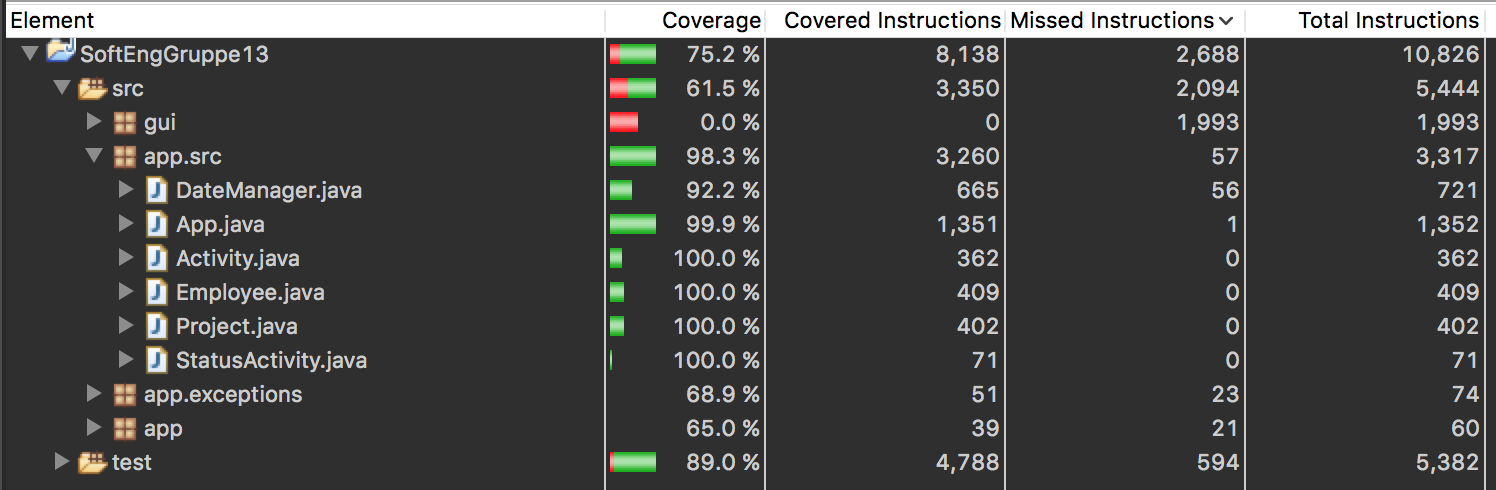
\includegraphics[width = \textwidth]{Figurer/CodeCoverage}
    \caption{Code coverage for programmet under præsentationslaget.}
    \label{fig:eclemma}
\end{figure}

Som det kan ses i figur \ref{fig:eclemma}, er der en 98.3 \% code coverage på source filerne (i \texttt{app.src} pakken). Den manglede dækning kommer fra \texttt{App} og \texttt{DateManager}. Som det kan ses er programmet testet under præsentationslaget med JUnit teste, hvor præsentationslaget selv er testet med manuelle teste.

I \texttt{App}'s konstruktør findes en try catch, hvor der aldrig vil blive fanget en exception, da prøvedataen er sat op, så den ikke kan fejle. Derfor er code coverage lavere end 100 \%. Alternativt kunne man sætte konstruktøren til at kaste en exception og håndtere den når man initialiserer objektet i vores \texttt{View}. \\

I \texttt{DateManager} findes metoder der returnerer en streng med information om den nuværende dato. Disse skal have den korrekte længde; hvis det er den første uge i året, skal strengen hedde "01". Da disse er sat til at opdatere datoen (initialisere et nyt \texttt{GregorianCalendar} objekt) hver gang en sådan metode bliver kaldt, vil der ikke altid blive tilføjet nuller til strengen. Dermed vil koden ikke blive kørt, når vi kommer længere ind i året.
De første 7 dage af året vil \texttt{DateManager} have fuld code coverage. Alternativt ville det være muligt at mocke den gregorianske kalender hver gang man opdaterer datoen, og styre testen derigennem for at få 100 \% code coverage. \\

Nu da der er (næsten) fuld code coverage, er der stor sandsynlighed for at programmet virker efter hensigten. Det er ikke garanteret at et program er korrekt bare fordi der er fuld code coverage. Selvom al koden bliver kørt under tests, skal testene også være konstrueret korrekt, for at sikre at resultatet af at køre koden også er som forventet. Derfor er det også vigtigt at vi udfører white box og black box testing af de essentielle dele af programmet.

